\chapter{Describes las relaciones trigonométricas para resolver triángulos rectángulos}

\section{Sistema sexagesimal y circular}

\subsection{Definicíon}

Para medir un ángulo, un grado representa $\frac{1}{360}$ de una
circunferiancia. Un minuto representa $\frac{1}{60}$ de un grado y un segundo
$\frac{1}{60}$ de un minuto. Por ejemplo un ángulo de 1° 9' 18'' representa
$\frac{1}{360} + 9 \times \frac{1}{360 \times 60} + 18 \times \frac{360 \times 60 \times 60} = \frac{77}{24000}$ de una circunferiancia. Eso es llamado el
sistema sexagesimal.

En ciencia, el sistema circular es más utilizado. Es definido tal que si un
ángulo $\alpha$ mide un radián, la longitud del arco corespondiente en
un círculo de radio $R$ sólo es $\alpha \times R$. Entonces, la medida de una
circunferencia corresponde a $2\pi \text{rad}$, la medida de una
semicircunferencia es $\pi \text{rad}$, la medida de un cuarto de la
circunferencia es $\frac{\pi}{2} \text{rad}$ etc

\subsection{Ejercicio 1}

\begin{enumerate}
\item Indique la valor en grado, minuto y segundo de un ángulo de $15.75$° y
  y $78.51$°.
\item Indique una approximación la medida en grado/minuto/segundo de un ángulo
  de 1 radián.
\item Exprese en función de $\pi$, la medida en radián de los ángulos de
  30°, 45°, 60°, 90°, 135°, 180°, 270° y 360°.
\item Exprese la formula de la área de un sector de $\alpha$ radianes para
  un círculo de radio $R$.
\end{enumerate}

\section{Funciones trigonométricas}

\subsection{Definicíon}

Consideramos un triángulo rectangulo y $\alpha$ la medida de un ángulo en
radián ($0 \leq \alpha < \frac{\pi}{2}$).

\begin{center}
 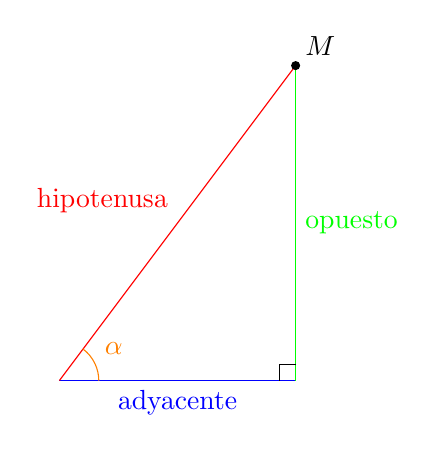
\begin{tikzpicture}
   \draw[color=blue] (0,0) -- (1.5,0)node[below]{adyacente} -- (3,0);
   \draw[color=green] (3,0) -- (3,2)node[right]{opuesto} -- (3,4);
   \draw[color=red] (3,4) -- (1.5,2)node[above left]{hipotenusa} -- (0,0);
   \draw (2.8,0) -- (2.8,.2) -- (3,.2);
   \draw[color=orange] (0.5,0) arc(0:25:.5) node[above right]{$\alpha$}
   arc(25:53.13010235415599:.5);
   \draw[fill=black] (3,4) node[above right]{$M$} circle(.05);
 \end{tikzpicture}
\end{center}

Esos ángulos recto y $\alpha$ determinan la clase de semejanza del
triángulo y por lo tanto los cocientes siguientes:

$$
\sin \alpha = \frac{\color{green}{\text{opuesto}}}
{\text{\color{red}{\text{hipotenusa}}}}
$$
%%
$$
\cos \alpha = \frac{\color{blue}{\text{adyacente}}}
{\text{\color{red}{\text{hipotenusa}}}}
$$
%%
$$
\tan \alpha = \frac{\color{green}{\text{opuesto}}}
{\text{\color{blue}{\text{adyacente}}}}
$$

Cuando $\alpha$ se acerca del ángulo recto $\frac{\pi}{2}$, la longitud
del lado opuesto se acerca de la longitud del hipotenusa y la longitud
del lado adyacente se acerca de 0. Por lo tanto, definimos
%%
$$
\cos \frac{\pi}{2} = 0
$$
%%
$$
\sin \frac{\pi}{2} = 1
$$
%%
pero no definimos $\tan$ en $\frac{\pi}{2}$, porque el cociente
$\frac{\color{green}{\text{opuesto}}}
{\text{\color{blue}{\text{adyacente}}}}$ se vuelve más en más grande cuando
$\alpha$ se acerca de $\frac{\pi}{2}$.

Podemos genaralizar las formulas precedientes si utilizamos valores
relativas para
$\color{green}{\text{opuesto}}$ y ${\text{\color{blue}{\text{adyacente}}}}$
según las coordenadas del vértice $M$ opuesto al ángulo $\alpha$:

$$\cos{(-\alpha)} = \cos{(\alpha)}$$
$$\sin{(-\alpha)} = -\sin{(\alpha)}$$
$$\tan{(-\alpha)} = -\tan{(\alpha)}$$
$$\cos{(\pi-\alpha)} = -\cos{(\alpha)}$$
$$\sin{(\pi-\alpha)} = \sin{(\alpha)}$$
$$\tan{(\pi-\alpha)} = -\tan{(\alpha)}$$

Finalmente hacer una vuelta $2\pi$ no debe cambiar los cocientos y entonces
la funciones deben ser periódicas (el ejercico 3 da un mejor resultado para
tangente):

$$\cos{(\alpha+2\pi)} = \cos{(\alpha)}$$
$$\sin{(\alpha+2\pi)} = \sin{(\alpha)}$$
$$\tan{(\alpha+2\pi)} = \tan{(\alpha)}$$

Esas formulas definen las funciones seno y coseno para todo
$\alpha \in \mathbb R$ y la función tangente sobre todo
$\alpha \in \left]{-\frac{\pi}{2} + k\pi}, {\frac{\pi}{2} +k\pi} \right[$
para $k \in \mathbb Z$. 

\subsection{Ejercicio 2}

\begin{enumerate}
  \item ¿Cuál es el seno, coseno y tangente de $\alpha=0$?
  \item Determine el ángulo $\alpha$ en un triángulo rectángulo isoceles
    así que el seno, coseno y tangente de $\alpha$.
  \item Consideramos un triángulo equilatero $ABC$ y sea $D$ el medio
    de $[BC]$. Muestre que $ABD$ es rectángulo en $D$ y determine sus
    ángulos $\widehat{A}$ y $\widehat{B}$ así que sus seno, coseno y
    tangente de los ángulos.
  \item Expresar los seno, coseno y tangente de $\frac{\pi}{6}$ y
    $\frac{\pi}{4}$ así que de sus múltiplos.
\end{enumerate}

\subsection{Ejercicio 3}

Muestre las igualidas siguientes para $0 \leq \alpha < \frac{\pi}{2}$:

\begin{enumerate}
\item Utilice $\alpha + \pi = -\left(\pi-\alpha\right) + 2\pi$ para determinar
  $\cos\left(\alpha+\pi\right)$ y $\sin\left(\alpha+\pi\right)$.
\item $\tan \alpha = \frac{\sin \alpha}{\cos \alpha}$. Deduzca que 
  $\tan \left(\alpha+\pi\right)$.
\item $\left(\sin \alpha\right)^2 + \left(\cos \alpha\right)^2 = 1$
\end{enumerate}

\subsection{Ejercicio 4}

\begin{enumerate}
\item Determine $\cos \frac{4\pi}{5}$ (respectivamente $\sin \frac{4\pi}{5}$)
  en functión de $\cos \frac{\pi}{5}$ (respectivamente $\sin \frac{\pi}{5}$)
  utilizando la formulas del coseno (respectivamente seno) para
  $\pi - \alpha$.
\item En la figura siguiente, determine todos los ángulos y 
  longitud y deduzca las formulas:

$$
{\sin {2\alpha}} = {2 {\sin \alpha} {\cos \alpha}}
$$
%%
$$
{\cos {2\alpha}} = {2 \left(\cos \alpha\right)^2 - 1}
$$

\begin{center}
 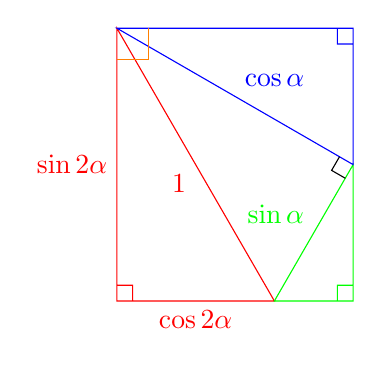
\begin{tikzpicture}
   \draw[color=red] (0,0) -- (1,0)node[below]{$\cos {2\alpha}$} --  (2,0) --
   (1,1.732050807568877)node[below left]{$1$} --
   (0,3.464101615137754) -- (0,1.732050807568877)node[left]{$\sin {2\alpha}$} --
   cycle (.2,0) -- (.2,.2) -- (0,.2);
   \draw[color=green] (2,0) -- (3,0) -- (3,1.732050807568877) -- 
   (2.5,0.86602540378443)node[above left]{$\sin \alpha$} -- cycle
   (2.8,0) -- (2.8,.2) -- (3,.2);

   \draw[color=blue] (3,1.732050807568877) -- (3,3.464101615137754) --
   (0,3.464101615137754) -- 
   (1.5,2.598076211353315)node[above right]{$\cos \alpha$} -- cycle
   (2.8,3.464101615137754) -- (2.8,3.264101615137754) -- (3,3.264101615137754);
   \draw[color=orange]
   (.4,3.464101615137754) -- (.4,3.064101615137754) -- (0,3.064101615137754);
   \begin{scope}[rotate around={-30:(3,1.732050807568877)}]
   \draw (2.8,1.732050807568877) -- (2.8,1.532050807568877) --
   (3,1.532050807568877);
   \end{scope}
 \end{tikzpicture}
\end{center}

\item Sea $x = \cos \frac{\pi}{5}$. Tenemos $0 < x < 1$.
 Utilice las formulas de la pregunta precediente para mostrar
%%
$$
{\sin \left(\frac{4\pi}{5}\right)} = 4 x \left(2x^2-1\right) \sin\left(\frac{\pi}{5}\right)
$$
%%
$$
{\cos \left(\frac{4\pi}{5}\right)} = 2 \left(2x^2 - 1\right)^2 - 1
$$

\item Muestre que $4x^2 - 2x -1 = 0$ y deducir
  $$
  {\cos \left(\frac{2\pi}{5}\right)} = \frac{\sqrt{5}-1}{4}
  $$
  Compare con la construción del pentágono regular en el ejercicio 6 del
  capítulo IV.

\end{enumerate}

\section{Resolución de triángulos rectángulos}

\subsection{Definición}

Si fijamos la longitud de la hipotenusa y movemos el punto $M$ en la parte
del plano tal que $0 \leq \alpha < \frac{\pi}{2}$,
las límites de los lados opuesto y adyacente son
%%
$$0 \leq {\color{green}{\text{opuesto}}} \leq {\color{red}{\text{hipotenusa}}}$$
$$0 \leq {\color{blue}{\text{adyacente}}} \leq {\color{red}{\text{hipotenusa}}}$$

\begin{center}
 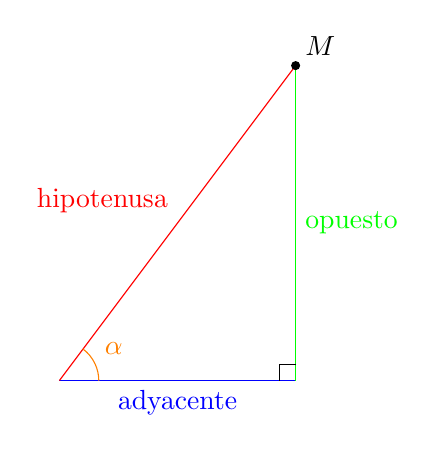
\begin{tikzpicture}
   \draw[color=blue] (0,0) -- (1.5,0)node[below]{adyacente} -- (3,0);
   \draw[color=green] (3,0) -- (3,2)node[right]{opuesto} -- (3,4);
   \draw[color=red] (3,4) -- (1.5,2)node[above left]{hipotenusa} -- (0,0);
   \draw (2.8,0) -- (2.8,.2) -- (3,.2);
   \draw[color=orange] (0.5,0) arc(0:25:.5) node[above right]{$\alpha$}
   arc(25:53.13010235415599:.5);
   \draw[fill=black] (3,4) node[above right]{$M$} circle(.05);
 \end{tikzpicture}
\end{center}

y entonces
%%
$$
0\leq \sin \alpha \leq 1
$$
$$
0\leq \cos \alpha \leq 1
$$

Recíprocamente un real $0 \leq x \leq 1$ determina un único triángulo rectángulo
${\color{blue}{\text{adyacente}}} = x$,
${\color{green}{\text{opuesto}}} = \sqrt{1-x^2}$ y
${\color{red}{\text{hipotenusa}}} = 1$ y entonces un único ángulo
$0 \leq \alpha_1 \leq \frac{\pi}{2}$. Definimos
%%
$$
\alpha_1 = \arccos x
$$

De la misma manera, un real $0 \leq x \leq 1$ determina un único triángulo
rectángulo ${\color{green}{\text{opuesto}}} = x$,
${\color{blue}{\text{adyacente}}} = \sqrt{1-x^2}$ y
${\color{red}{\text{hipotenusa}}} = 1$ y entonces un único ángulo
$0 \leq \alpha_2 \leq \frac{\pi}{2}$. Definimos
%%
$$
\alpha_2 = \arcsin x
$$

Ahora fijamos la longitud del lado adyacente y movemos el punto $M$ en la parte
del plano tal que $0 \leq \alpha < \frac{\pi}{2}$. $M$ puede mover
verticálamente y la longitud de
${\color{green}{\text{opuesto}}}$ puede ir de $0$ a una
valor tan grande como queremos. Un real $x \geq 0$, determina un
únique triangulo ${\color{green}{\text{opuesto}}} = x$,
${\color{blue}{\text{adyacente}}} = 1$ y
${\color{red}{\text{hipotenusa}}} = \sqrt{1+x^2}$ y entonces un 
único ángulo $0 \leq \alpha_3 < \frac{\pi}{2}$. Definimos
%%
$$
\alpha_3 = \arctan x
$$

Las functiones seno, coseno, tangente, arcocoseno,  arcoseno y arcotangente
son disponible en calculadoras, lo que permite resolver triángulos rectángulos
conociendo dos parámetros (lado o ángulo no recto).

\subsection{Ejercicio 5}

Sea $ABC$ un triángulo rectángulo en $A$. Determine una aproximación de

\begin{enumerate}
\item la longitud $BC$ si $\widehat{C} = 15°$ y $AC = 10\text{cm}$.
\item la amplitud del ángulo $\widehat{B}$ si $AC = 5\text{cm}$ y
  $BC = 8\text{cm}$.
\item la amplitud de $AB$ si $AC = 8\text{cm}$ y $\widehat{B} = 65°$.
\item la longitud $AB$ si $BC = 15\text{cm}$ y $\widehat{B} = 55°$.
\end{enumerate}

\section{Soluciones de los ejercicios }

\subsection{Ejercicio 1}

\begin{enumerate}
\item 15°45' y 78°30'36''
\item $1 \text{rad} = \frac{360}{2\pi} = \frac{180}{\pi} \approx
  57°17'45''$.
\item $\frac{\pi}{6}, \frac{\pi}{4}, \frac{\pi}{3}, \frac{\pi}{2}, 
  \frac{3\pi}{8}, \pi, \frac{3\pi}{2}, 2\pi$.
\item $\frac{\alpha}{2} R^2$
\end{enumerate}

\subsection{Ejercicio 2}

\begin{enumerate}
\item Cuando $\alpha=0$, ${\color{green}{\text{opuesto}}} = 0$ y
  ${\color{blue}{\text{adyacente}}} = \text{\color{red}{\text{hipotenusa}}}$
  entonces ${\tan 0} = {\sin 0} = 0$ y $\cos 0 = 1$.
\item Para un triángulo rectángulo isoceles, $\frac{\pi}{2} + \alpha + \alpha = \pi$ entonces $\alpha = \frac{\pi}{4} = 45°$. Si $x$ es la longitud de los catetos, tenemos ${\color{green}{\text{opuesto}}} = {\color{blue}{\text{adyacente}}} = x$ y por el teorema de Pítagora $\text{\color{red}{\text{hipotenusa}}} = 
x \sqrt{2} $. Entonces $\sin \frac{\pi}{4} = \cos \frac{\pi}{4} = \frac{x}{x \sqrt{2}} = \frac{\sqrt{2}}{2}$ y $\tan \frac{\pi}{4} = 1$.
\item Sea $x$ la longitud de de los lados del triángulo rectángulo equilatero
  $ABC$: ${AB} = {AC} = {BC} = x$.
  $D$ es el medio de $[BC]$ entonces ${AD} = \frac{BC}{2} = \frac{x}{2}$.
  Además, por que $A, D$ son sobre la mediatriz de $[BC]$ y entonces
  $ABD$ es rectángulo en $D$ (es decir $\widehat{D} = \frac{\pi}{2}$).
  Por el teorema de Pítagoras, 
  $AD = \sqrt{x^2 - \left(\frac{x}{2}\right)^2} = \frac{\sqrt{3}}{2} x$.
  $ABC$ es equilatero y entonces $\widehat{B} = \frac{\pi}{3} = 60°$ y
  $\widehat{A} = \pi - \widehat{D} - \widehat{B} = \frac{\pi}{6}$.
  Finalmente, 
  $\sin \widehat{A} = \cos \widehat{B} = \frac{x/2}{x} = \frac{1}{2}$
  $\cos \widehat{A} = \sin \widehat{B} = \frac{\frac{\sqrt{3}}{2} x}{x} =
  \frac{\sqrt{3}}{2}$,
  $\tan \widehat{A} = \frac{\sqrt{3}}{3}$ y
  $\tan \widehat{B} = \sqrt{3}$.
\item Ya hamos obtenido los valores para $\alpha = 0, \frac{\pi}{6}, \frac{\pi}{4}, \frac{\pi}{3}, \frac{\pi}{2}$. Utilizando las simétrias de las funciones
  trigonometrías, podemos deducir las valores para los multíplios de eso
  ángulos.

  \begin{center}
  \begin{tabular}{| l | c | c | c | c | c | c | c | c | c | c | c | c | c | c | c | c |}
    \hline
    $\alpha$ &
    $-\frac{5\pi}{6}$ &
    $-\frac{3\pi}{4}$ &
    $-\frac{2\pi}{3}$ &
    $-\frac{\pi}{2}$ &
    $-\frac{\pi}{3}$ &
    $-\frac{\pi}{4}$ &
    $-\frac{\pi}{6}$ &
    $0$ &
    $\frac{\pi}{6}$ &
    $\frac{\pi}{4}$ &
    $\frac{\pi}{3}$ &
    $\frac{\pi}{2}$ &
    $\frac{2\pi}{3}$ &
    $\frac{3\pi}{4}$ &
    $\frac{5\pi}{6}$ &
    $\pi$ \\
    \hline
    $\sin \alpha$ & 
    $-\frac{1}{2}$ &
    $-\frac{\sqrt{2}}{2}$ &
    $-\frac{\sqrt{3}}{2}$ &
    $-1$ &
    $-\frac{\sqrt{3}}{2}$ &
    $-\frac{\sqrt{2}}{2}$ &
    $-\frac{1}{2}$ &
    $0$ &
    $\frac{1}{2}$ &
    $\frac{\sqrt{2}}{2}$ &
    $\frac{\sqrt{3}}{2}$ &
    $1$ &
    $\frac{\sqrt{3}}{2}$ &
    $\frac{\sqrt{2}}{2}$ &
    $\frac{1}{2}$ &
    $0$
    \\
    \hline
    $\cos \alpha$ &
    $-\frac{\sqrt{3}}{2}$ &
    $-\frac{\sqrt{2}}{2}$ &
    $-\frac{1}{2}$ &
    $0$ &
    $\frac{1}{2}$ &
    $\frac{\sqrt{2}}{2}$ &
    $\frac{\sqrt{3}}{2}$ &
    $1$ &
    $\frac{\sqrt{3}}{2}$ &
    $\frac{\sqrt{2}}{2}$ &
    $\frac{1}{2}$ &
    $0$ &
    $-\frac{1}{2}$ &
    $-\frac{\sqrt{2}}{2}$ &
    $-\frac{\sqrt{3}}{2}$ &
    $-1$
    \\
    \hline
    $\tan \alpha$ & 
    $\frac{\sqrt{3}}{3}$ &
    $1$ &
    $\sqrt{3}$ &
    / &
    $-\sqrt{3}$ &
    $-1$ &
    $-\frac{\sqrt{3}}{3}$ &
    $0$ &
    $\frac{\sqrt{3}}{3}$ &
    $1$ &
    $\sqrt{3}$ &
    / &
    $-\sqrt{3}$ &
    $-1$ &
    $-\frac{\sqrt{3}}{3}$ &
    $0$
    \\
    \hline
  \end{tabular}
  \end{center}
  
\end{enumerate}

\subsection{Ejercicio 3}

\begin{enumerate}
\item $\cos \left(\alpha + \pi\right) =
  \cos \left(-\left(\pi-\alpha\right) + 2\pi\right) = 
  \cos \left(-\left(\pi-\alpha\right)\right) =
  \cos \left(\left(\pi-\alpha\right)\right) = -\cos(\alpha)$ y 

$\sin \left(\alpha + \pi\right) =
  \sin \left(-\left(\pi-\alpha\right) + 2\pi\right) = 
  \sin \left(-\left(\pi-\alpha\right)\right) =
  -\sin \left(\left(\pi-\alpha\right)\right) = -\sin(\alpha)$
\item $\frac{\sin \alpha}{\cos \alpha} =
\frac{\frac{\color{green}{\text{opuesto}}}{\text{\color{red}{\text{hipotenusa}}}}}{\frac{\color{blue}{\text{adyacente}}}{\text{\color{red}{\text{hipotenusa}}}}} = 
\frac{\color{green}{\text{opuesto}}}{\color{blue}{\text{adyacente}}} =
{\tan \alpha}$. Entonces, 
$\tan \left(\alpha+\pi\right) = \frac{-\sin \alpha}{-\cos \alpha} =
\frac{\sin \alpha}{\cos \alpha} = {\tan \alpha}$.

\item $\left(\sin \alpha\right)^2 + \left(\cos \alpha\right)^2 = 
  \frac{{\color{green}{\text{opuesto}}}^2
    +{\color{blue}{\text{adyacente}}}^2
  }{\text{\color{red}{\text{hipotenusa}}}^2} = 1$ por el teorema de Pítagoras.
\end{enumerate}

\subsection{Ejercicio 4}

\begin{enumerate}
\item
  $$\cos\left(\frac{4\pi}{5}\right) = \cos\left(\pi-\frac{\pi}{5}\right) =
  -\cos\left(-\frac{\pi}{5}\right) = -\cos\left(\frac{\pi}{5}\right)$$
  $$\sin\left(\frac{4\pi}{5}\right) = \sin\left(\pi-\frac{\pi}{5}\right) =
  -\sin\left(-\frac{\pi}{5}\right) = \sin\left(\frac{\pi}{5}\right)$$

\item En el triángulo rectángulo rojo, el ángulo adyacente al lado de longitud 
  $\cos 2\alpha$ mide $2\alpha$ y el ángulo opuesto $\frac{\pi}{2} - 2\alpha$.
  De la misma manera, en el triángulo rectángulo central, el ángulo adyacente
  al lado de longitud $\cos \alpha$ mide $\alpha$ y el ángulo opuesto
  $\frac{\pi}{2} - \alpha$. Por lo tanto, dedicimos los ángulos que tocan
  esos ángulos en el triángulo rectángulo azul ($\frac{\pi}{2} -
  \left(\frac{\pi}{2} - 2\alpha\right) - \alpha =
  \alpha$) y verde ($\pi - 2\alpha - \left(\frac{\pi}{2}-\alpha\right) =
  \frac{\pi}{2} - \alpha$).
  Finalmente, obtenemos los ángulos que tocan el ángulo recto del
  triángulo central: $\frac{\pi}{2} - \alpha$ (triángulo ázul) y $\alpha$
  (triángulo verde) y podemos verifiar que suman 180° con el ángulo recto
  del triángulo central.

  Los lados del triángulo ázul son $\left(\cos \alpha\right)^2$ (horizontal) y
  ${\sin \alpha} {\cos \alpha}$ (vertical). 
  Los lados del triángulo verde son $\left(\sin \alpha\right)^2$ (horizontal) y
  ${\sin \alpha} {\cos \alpha}$ (vertical). Finalmente,
%%
  $${\sin \left(2\alpha\right)} = 2 {\sin \alpha} {\cos \alpha}$$
%%
  $${\cos \left(2\alpha\right)} = \left(\cos \alpha\right)^2 - 
  \left(\sin \alpha\right)^2 = 
  2\left(\cos \alpha\right)^2 - 1$$
%%  
  donde hemos utilizado la formula del ejercicio 3 para simplificar
  $\cos \left(2\alpha\right)$.

\item 

${\sin \left(\frac{4\pi}{5}\right)} = 2 {\sin \left(\frac{2\pi}{5}\right)}
{\cos \left(\frac{2\pi}{5}\right)}$ y
${\cos \left(\frac{4\pi}{5}\right)} =
2 \left({\cos \left(\frac{2\pi}{5}\right)}\right)^2 - 1$. Moreover,
${\sin \left(\frac{2\pi}{5}\right)} = 2 x {\sin \left(\frac{\pi}{5}\right)}$ y
${\cos \left(\frac{2\pi}{5}\right)} = 2x^2 - 1$.

\item Porque
$\sin\left(\frac{4\pi}{5}\right) = \sin\left(\frac{\pi}{5}\right) \neq 0$,
la primera equalidad se vuelve
%%
$$2 \left(2x^2-1\right) = \frac{1}{2x}$$

Y porque $\cos\left(\frac{4\pi}{5}\right) = -\cos\left(\frac{\pi}{5}\right) = -x$ la segunda equalidad se vuelve
%%
$$2\left(2x^2-1\right)^2 = 1 - x$$

Si tomamos el cociente de la segunda por la primera, obtenemos
%%
$$
2x^2 - 1 = {2x\left(1 - x \right)} = 2x - 2x^2
$$
%%
y entonces
%%
$$
4x^2 - 2x - 1 = 0
$$

La solución positiva de esta ecuacion es $x = \frac{2 + \sqrt{4+16}}{8} = 
\frac{1+\sqrt{5}}{4}$ y finalmente
%%
  $$
  {\cos \left(\frac{2\pi}{5}\right)} = {2x^2 - 1} = \frac{\sqrt{5}-1}{4}
  $$

\end{enumerate}

\subsection{Ejercicio 5}

\begin{enumerate}
\item $BC = \frac{AC}{\cos 15°} \approx 10.36\text{cm}$.
\item $\widehat{B} = \arcsin \frac{5}{8} \approx 38°41'$
\item $AB = \frac{AC}{\tan 65°} \approx 18.93\text{cm}$.
\item $AB = BC {\cos 55°} \approx 8.60\text{cm}$.
\end{enumerate}
